\section{Background}

\noindent\textbf{Basic Fuzzy Logic:} Basic Fuzzy Logic (BL)  is a relaxation of first-order logic that operates on continuous truth
values on the interval [0, 1] instead of on boolean values. BL
uses a class of functions called \textit{t-norms} ($\otimes$), which preserves
the semantics of boolean conjunctions on continuous truth
values. Formally, a t-norm is defined $\otimes$ : $[0, 1] \times [0, 1] \rightarrow [0, 1]$ such that:
\begin{itemize}
    \item $\otimes$ is consistent for any $t \in [0, 1]:$ 

            \quad \quad \quad  $$t \otimes 1 = t \quad\quad t \otimes 0 = 0$$
    % \item \otimes \text{is commutative and associative for any t \in [0, 1]:} $$ t_{1} \otimes t_{2} = t_{2} \otimes t_{1} \quad t_{1} \otimes (t_{2} \otimes t_{3}) = (t_{1} \otimes t_{2}) \otimes t_{3} $$
\end{itemize}

\begin{itemize}
    \item $\otimes$ \text{is commutative and associative for any $t \in [0, 1]$:} 
    
        $$ t_{1} \otimes t_{2} = t_{2} \otimes t_{1} \quad t_{1} \otimes (t_{2} \otimes t_{3}) = (t_{1} \otimes t_{2}) \otimes t_{3} $$
\end{itemize}

\begin{itemize}
    \item $\otimes$ is monotonic (non decreasing) for any $t \in [0, 1]$:

        $$ t_{1} \leq t_{2} \implies t_{1} \otimes t_{3} \leq t_{2} \otimes t_{3} $$
\end{itemize}

\begin{table*}[t]
\begin{tabular*}{\textwidth}{c @{\extracolsep{\fill}} cccc}
  & Lukaseiwicz: & Godel: & Product: \\ 
 tnorm ($\otimes$) & $max(0, t + u − 1)$ & $min(t, u)$ & $t * u$ \\  
 tconorm ($\oplus$) & $min(t + u, 1)$ & $max(t, u)$ & $t + u - t * u$
\end{tabular*}
\caption{}
\label{tab:tnorms}
\end{table*}

\noindent BL additionally requires that t-norms be continuous. \textit{T-conorms} ($\oplus$) are derived from t-norms via DeMorgan’s law and operate as disjunctions on continuous truth values, while negations are defined $\neg{t} := 1 - t$.

\noindent Three widely used t-norms that satisfy the requirements are the
Lukaseiwicz t-norm \cite{luka}, the Godel t-norm \cite{baaz1996} and the product t-norm \cite{hajek1996}. Each t-norm has a \textit{t-conorm} associated with it (denoted $\oplus$), which can be
considered as logical disjunction. Given a t-norm $\otimes$, the t-conorm can be derived with DeMorgan’s
law: $t \oplus u$ $\overset{\Delta}{=}$ $\neg{(\neg{t} \otimes \neg{u})}$. Table \ref{tab:tnorms} shows the formule for tnorms and tconorms.

% \centering


\noindent\textbf{Gated t-norms and gated t-conorms:} Given a classic t-norm $T(x, y) = x \otimes y$, we define its associated gated t-norm as 

$$T_{G}(x,y;g_{1},g_{2}) = (1 + g_{1}(x - 1)) \otimes (1 + g_{2}(y - 1))$$

Here $g_{1}, g_{2} \in [0, 1]$ are gate parameters indicating if x and y are activated, respectively.

\[
    T_{G}(x,y;g_{1},g_{2})= 
\begin{cases}
    x \otimes y & g_{1} = 1 \hspace{2mm} \text{and} \hspace{2mm} g_{2} = 1\\
    x & g_{1} = 1 \hspace{2mm} \text{and} \hspace{2mm} g_{2} = 0\\
    y & g_{1} = 0 \hspace{2mm} \text{and} \hspace{2mm} g_{2} = 1\\
    1 & g_{1} = 0 \hspace{2mm} \text{and} \hspace{2mm} g_{2} = 0
\end{cases}
\]

Using DeMorgan’s laws $x \otimes y = 1 - (1 - x) \otimes (1 - y)$, we define gated t-conorms as

$$T_{G}^{'}(x,y;g_{1},g_{2}) = 1 - (1 - g_{1}x) \otimes (1 - g_{2}y)$$,

and has following property - 
\[
    T_{G}^{'}(x,y;g_{1},g_{2})= 
\begin{cases}
    x \otimes y & g_{1} = 1 \hspace{2mm} \text{and} \hspace{2mm} g_{2} = 1\\
    x & g_{1} = 1 \hspace{2mm} \text{and} \hspace{2mm} g_{2} = 0\\
    y & g_{1} = 0 \hspace{2mm} \text{and} \hspace{2mm} g_{2} = 1\\
    0 & g_{1} = 0 \hspace{2mm} \text{and} \hspace{2mm} g_{2} = 0
\end{cases}
\]

\noindent\textbf{Continuous Logic Network (CLN):} CLN's are based on parametric relaxation Logical formulas that maps the logical formulation from boolean first order logic to BL.
The model defines the operator \script{S}. A quantifier-free boolean formula $F: X \rightarrow {True, False}$, \script{S} maps it to a continuous function $\script{S}(F): X \rightarrow [0, 1]$. In order for the continuous model to be both usable in gradient-guided optimization while also preserving the semantics of boolean
logic, it must fulfill three conditions:

\begin{enumerate}
    \item It must preserve the meaning of the logic, such that the continuous truth values of a valid assignment are always greater than the value of an invalid assignment:
        \begin{dmath}(F(x) = True \wedge F(x') = False) \implies \script{S}(F)(x) > \script{S}(F)(x')\end{dmath}
    \item It must be must be continuous and smooth (i.e. differentiable almost everywhere) to facilitate training.
    \item It must be strictly increasing as an unsatisfying assignment of terms approach satisfying the mapped formula,
and strictly decreasing as a satisfying assignment of
terms approach violating the formula.
\end{enumerate}

\script{S} is constructed as follows to satisfy these requirements. The
logical relations {$\wedge, \lor, \lnot$} are mapped to their continuous
equivalents in BL:

$$Conjunction: \script{S}(F_{1} \wedge F_{2}) \triangleq \script{S} F_{1} \otimes F_{2}$$
$$Disjunction: \script{S}(F_{1} \lor \F_{2}) \triangleq \script{S} F_{1} \otimes F_{2}$$
$$Negation: \script{S}(\neg{F}) \triangleq 1 - \script{S}(F)$$

For Gated CLN, we use gated t-norms and gated t-conorms.
%% ----------------- DEEPSYNTH PART -----------------
% \subsection{DeepSynth's Neural Network Architecture}
% \label{dgnn}
% This part explains the neural network architecture and training data generation techniques used in deepsynth and how are these integrated together.

% \begin{figure*}
%     \centering
%     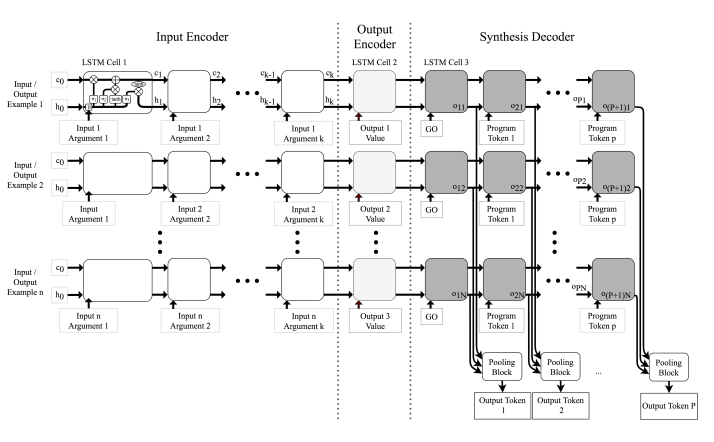
\includegraphics[scale=0.5]{DSNN.png}
%     \caption{The DeepSynth Neural Network}
%     \label{fig:dsnn}
% \end{figure*}

% \subsubsection{Neural Network}
% The DeepSynth Neural Network, shown in Fig. \ref{fig:dsnn} is made up of several parallelised sequence-to-sequence neural networks, each of which processes a single counterexample (i.e. I/O example) and computes a probability distribution over the likely sequence of tokens in the program given that input/output example. The outputs from all the sequence-to-sequence networks are combined using pooling. In the following sections we describe in detail a single sequence-to-sequence network, and then the pooling process.

% \paragraph{Processing a Single counterexample}
% \begin{figure*}
%     \centering
%     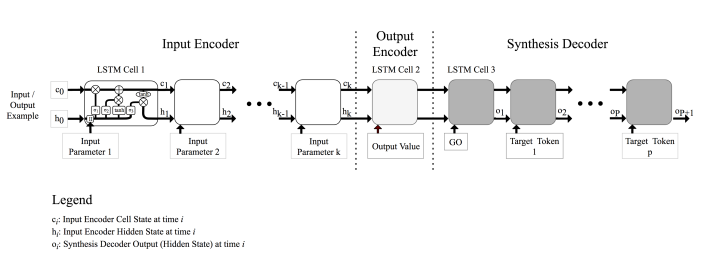
\includegraphics[scale=0.5]{dsnn2.png}
%     \caption{Seq2Seq network for a single I/O example}
%     \label{fig:dsnn2}
% \end{figure*}
% The Seq2Seq network used for processing a single counterexample is shown in Fig. \ref{fig:dsnn2} and consists of:
% \begin{enumerate}
%     \item An \textbf{input encoder} LSTM network, which receives the input argument values from the I/O example.
%     \item An \textbf{output encoder} LSTM cell, which receives the output value from the I/O example and is conditioned on the final cell and hidden states of the input encoder network.
%     \item A \textbf{synthesis decoder} LSTM network, which is trained on the \textbf{target program} and conditioned on the final output encoder state.
% \end{enumerate}
% Input arguments are fed into the input encoder network as a sequence. The cell state and hidden states of all three LSTM cells (for the input encoder, output encoder, and synthesis decoder respectively) are set to be 128-dimensional vectors. Program tokens are represented using a learnable 128-dimensional vector embedding. Every program token in the token vocabulary has a 128-dimensional vector representation which is updated at each time step of training.

% DeepSynth evaluates three different representations for input arguments and the output values, which is referred as \textbf{input-modes:}
% \begin{enumerate}
%     \item \textbf{"normalised"} mode, where every parameter value p is represented by a normalised scalar value, more specifically $\frac{p}{2^{31}} - 1$ \item \textbf{"binary"} mode, where p is provided in its binary representation, a 32-dimensional vector of 0s and 1s. This representation is more useful for helping the network detect minute differences between inputs.
%     \item \textbf{"normBinary"} mode, which combines both normalised and binary representations, thus producing a 33-dimensional vector representation for every input argument and the output value.
% \end{enumerate}

% Finally, it includes an additional setting for the network, in which the synthesis decoder is provided with the arity (i.e. number of input arguments) of the target program in addition to the target program’s tokens.

% \paragraph{Pooling}
% To process n I/O examples, the DeepSynth neural network creates n identical copies of the single-IO Seq2Seq network, with each receiving one of the n I/O examples. Once it has the encoded I/O examples, it is then fed to n synthesis decoders along with a GO token at time step 1, and a 128-dimensional hidden state is produced from each decoder. Let $o_{t_i}$ be the hidden state produced at time $t$ by synthesis decoder $i$. 

% To aggregate all hidden states $o_{T_i}$ at any given time T , these values are first passed through a \textbf{fully-connected neural network layer} to compute
% $n$ values ${fc}_{T_i}$ such that ${fc}_{T_i} = tanh(W * o_{T_i} + b)$, where W is a 128-by-128 weight matrix and b is a 128-by-1 bias matrix. Following this, the $n$ ${fc}_{T_i}$ values are aggregated into a unique 128-dimensional aggregate output value $O_T$ using the max pooling operation as follows: $$O_T[j] = \underset{1\le i \le n}{\mathrm{max}}{fc}_{T_i}[j]$$
% where $O_T[j]$ is the $j^{th}$ dimension of $O_T$ and ${fc}_{T_i}[j]$ is the $j^{th}$ dimension of ${fc}_{T_i}$. Finally, $O_T$ is used to compute the probability distribution $D_T$ over the next token using a softmax neural network layer. More formally, $D_T = softmax(W_{Lin} * O_T + b_{Lin})$, where $W_{Lin}$ is a 50-by-128 weight matrix and $b_{Lin}$ is a 50-by-1 bias vector (50 is the size of vocabulary). The pooling procedure is shown in Fig. \ref{fig:pool}
% \begin{figure*}
%     \centering
%     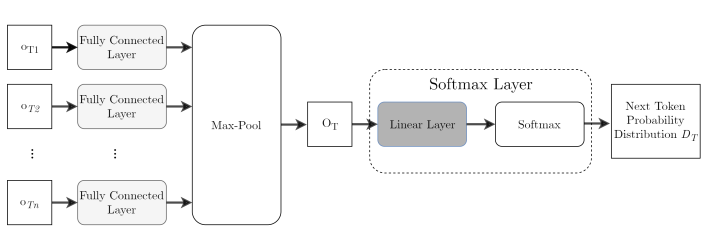
\includegraphics[scale=0.5]{pool.png}
%     \caption{The Pooling Operation}
%     \label{fig:pool}
% \end{figure*}

% \subsubsection{Training Data Generation}
% The Training Data consists of a set of Candidate programs, each accompanied by a corresponding set of input/output examples. For program synthesis, neural networks typically require millions of training examples therefore, in order to obtain a sufficiently large training data set, they designed a program generator that randomly generated programs made up of syntactically correct combinations of SYGUS-IF instructions \footnote{https://sygus.org/assets/pdf/SyGuS-IF\_2.0.pdf}. Randomly generated data set also consists of \textbf{"bad training data"} which is then pruned out using some set of rules and SMT based procedure.

% \noindent\textbf{Bad Training Data:} Redundant programs and input/output examples that do not sufficiently
% differentiate between programs. These are removed using following methods.

% \paragraph{Eliminating redundancy in programs}
% \noindent\textbf{Constants in programs} There are several cases where the choice of constants in programs can introduce redundancy. 
% \begin{itemize}
%     \item Shifting a bit vector by any number greater than the bit vector width produces a 0. Thus, a rule is introduced such that no generated program contains any shift operation with the second operand greater than the width of the first.
%     \item Zero value constants are disallowed in all cases since they almost always introduce redundancy.
% \end{itemize}

% \noindent\textbf{SMT based Redundancy Check} SMT-solver is used to identify two sources of redundancy:
% \begin{itemize}
%     \item An if-then-else statement is redundant when it always returns one of its conditional outputs. This redundancy is identified by recursively identifying leaf operators (i.e. operators not having nested ite statements) and checking their branch satisfiability with an SMT solver. If a branch is unreachable, the if-then-else statement is replaced with the other branch and call the recursive function again. This is continued until no leaf statements are redundant.
%     \item The SMT Solver also identifies  those programs that always return a single constant value, or always return a single one of the input arguments, and remove them from the training set.
% \end{itemize}

% \paragraph{Input/Output Example Generation}
% Input/Output examples are generated uniformly from a target program by executing the programs in order to get the corresponding outputs.

% DeepSynth generates Input/Output (I/O) examples for each random program such that this I/O is informative with respect to this program, i.e., the I/O must cover all conditional branches in a program so as to fully portray a program’s semantics. This is done by using a combination of randomly generated inputs and SMT solving. For a program P with C conditional statements and a shift assertion set S, “Smart” mode cycles through all $2^C$ possible execution cases and, where a case is satisfiable subject to S, it produces a new I/O example. This is done until N I/O examples are produced. In order to obtain a distribution of inputs over the input space when using an SMT solver, Z3 is used with the phase selection set to random.

% \paragraph{Program Tokenisation}
% Programs are converted into a \textbf{token} representation that the network can process. This representation encodes every operator in the DSL, as well as up to 10 different input parameters in a program, as its own token. Constants are each encoded using 8 tokens, such that each token represents a 4 bit value and can take on one of 16 values. 
% Two extra tokens are introduced for GO and EOS, which is used by the network during training to learn when synthesis starts/stops. To uniformise the length of its program sets, a PAD token is introduced. In total the vocabulary consists of 50 tokens for representing operations, input parameters, and constants that can appear in the program DSL.

% \paragraph{Batches} Programs’ token representations and I/O examples are aggregated into batches of size B. It also pads batch programs to one same length for computational reasons and converts I/O values into normalised and binary input format.
